\chapter{Параллельный перенос}
\label{chap:parallel-transport}

\section{Параллельные поля}

Пусть $\gamma\:[a,b]\z\to \Sigma$ --- гладкая кривая на гладкой поверхности $\Sigma$.
Гладкая векторнозначная функция $t\mapsto {\vec v}(t) \in \mathbb{R}^3$ называется \index{касательное!поле}\emph{касательным полем} вдоль $\gamma$, если
вектор ${\vec v}(t)$ лежит в касательной плоскости $\T_{\gamma(t)}\Sigma$ для любого~$t$.

Касательное поле ${\vec v}$ на кривой $\gamma$ называется \index{параллельные поле и перенос}\emph{параллельным}, если ${\vec v}'(t)\perp\T_{\gamma(t)}$ для любого~$t$.

В общем случае семейство касательных плоскостей $\T_{\gamma(t)}\Sigma$ не является параллельным.
Поэтому никак нельзя ожидать наличия \textit{по-настоящему} параллельного поля с ${\vec v}'(t)\equiv 0$ вдоль $\gamma$.
Условие ${\vec v}'(t)\z\perp\T_{\gamma(t)}$ значит, что поле старается вести себя как можно \textit{параллельней} --- ему приходится крутиться вместе с касательной плоскостью, но оно не крутится внутри оной.

По определению геодезической, поле скоростей ${\vec v}(t)\z=\gamma'(t)$ любой геодезической $\gamma$  параллельно вдоль~$\gamma$.

\begin{thm}{Упражнение}\label{ex:parallel}
Пусть $\gamma\:[a,b]\to \Sigma$ --- гладкая кривая на гладкой поверхности $\Sigma$, а ${\vec v}(t)$ и $\vec w(t)$ --- параллельные векторные поля вдоль~$\gamma$.

\begin{subthm}{ex:parallel:a}
Покажите, что величина $|{\vec v}(t)|$ постоянна.
\end{subthm}

\begin{subthm}{ex:parallel:b}
Покажите, что угол $\theta(t)=\measuredangle({\vec v}(t),\vec w(t))$ постоянен.
\end{subthm}

\end{thm}


\section{Параллельный перенос}

\begin{thm}{Предложение и определение}\label{prop:parallel}
Пусть $\gamma\:[a,b]\z\to \Sigma$ --- кусочно гладкая кривая на гладкой поверхности $\Sigma$,
и пусть $p\z=\gamma(a)$ и $q\z=\gamma(b)$.

Для данного касательного вектора ${\vec w}\in\T_p$ существует единственное параллельное такое поле ${\vec w}(t)$ вдоль $\gamma$, что ${\vec w}(a)={\vec w}$.

Вектор ${\vec w}(b)\in\T_q$ называется \index{параллельные поле и перенос}\emph{параллельным переносом} вектора ${\vec w}(a)$ вдоль~$\gamma$ на~$\Sigma$.
\end{thm}

Параллельный перенос вдоль $\gamma$ будет обозначаться как $\iota_\gamma$;
то есть можно писать $\vec w(b)=\iota_\gamma({\vec w}(a))$ или $\vec w(b)=\iota_\gamma({\vec w}(a))_\Sigma$, если нужно подчеркнуть, что $\gamma$ лежит на поверхности~$\Sigma$.
Из упражнения~\ref{ex:parallel} следует, что параллельный перенос $\iota_\gamma\:\T_p\z\to\T_q$ является изометрией.
В общем случае, параллельный перенос $\iota_\gamma\:\T_p\z\to\T_q$ зависит от выбора $\gamma$; то есть, для другой кривой $\gamma_1$, идущей из $p$ в $q$, параллельные переносы $\iota_{\gamma_1}$ и $\iota_{\gamma}$ могут различаться.

{\sloppy

\parbf{Идея доказательства.}
Предположим, что кривая $\gamma$ гладкая и она покрыта картой $(u,v)\mapsto s(u,v)$ поверхности $\Sigma$;
тогда $\gamma(t)\z=s(u(t),v(t))$ для гладких функций $t\mapsto u(t)$ и $t\mapsto v(t)$.
Определим 
\[
\vec u(t)=s_u(u(t),v(t)),
\quad
\vec v(t)=s_v(u(t),v(t)),
\quad
\text{и}
\quad
\Norm(t)=\Norm(\gamma(t)).
\]

}

Условия $\vec w(t)\in \T_{\gamma(t)}$ и $\vec w'(t)\perp \T_{\gamma(t)}$ записываются системой уравнений
\[
\begin{cases}
\ \langle\vec w(t), \Norm(t)\rangle=0,
\\
\ \langle\vec w'(t), \vec u(t)\rangle=0,
\\
\ \langle\vec w'(t), \vec v(t)\rangle=0.
\end{cases}
\]
Переписав эту систему через компоненты $\vec u$, $\vec v$, $\vec w$ и $\Norm$, получим систему обыкновенных дифференциальных уравнений на компоненты $\vec w$, и, применив \ref{thm:ODE}, получим решение $\vec w(t)$.
По \ref{ex:parallel}, $|\vec w(t)|$ не меняется;
следовательно, \ref{thm:ODE} влечёт, что решение $\vec w$ определено на всём интервале $[a,b]$.

Если $\gamma$ только кусочно гладкая или не покрыта одной картой, то можно её представить как произведение гладких дуг $\gamma_1,\dots,\gamma_n$ таких, что каждая $\gamma_i$ покрыта одной картой.
Последовательно применив предложение к каждой $\gamma_i$, получим его для $\gamma$.
\qeds


Предположим, что $\gamma_1$ и $\gamma_2$ --- две гладкие кривые на двух гладких поверхностях $\Sigma_1$ и $\Sigma_2$ со сферическими отображениями $\Norm_i\:\Sigma_i\to\mathbb{S}^2$.
Если $\Norm_1\circ\gamma_1(t)= \Norm_2\circ\gamma_2(t)$ для любого $t$, то будем говорить, что кривые $\gamma_1$ и $\gamma_2$ имеют \emph{идентичные нормали} на $\Sigma_1$ и $\Sigma_2$ соответственно.

В этом случае касательная плоскость $\T_{\gamma_1(t)}\Sigma_1$ параллельна касательной плоскости $\T_{\gamma_2(t)}\Sigma_2$ для любого~$t$, и можно отождествить $\T_{\gamma_1(t)}\Sigma_1$ с $\T_{\gamma_2(t)}\Sigma_2$.
В частности, если $\vec v(t)$ --- касательное поле вдоль $\gamma_1$,
то оно же и касательное вдоль $\gamma_2$.
Более того, $\vec v'(t)\perp \T_{\gamma_1(t)}\Sigma_1$ эквивалентно $\vec v'(t)\perp \T_{\gamma_2(t)}\Sigma_2$; то есть, если $\vec v(t)$ параллельно вдоль $\gamma_1$,
то оно параллельно и вдоль $\gamma_2$.

Рассуждение выше приводит к следующему наблюдению, которое скоро себя проявит.

\begin{thm}{Наблюдение}\label{obs:parallel=}
Пусть $\gamma_1$ и $\gamma_2$ --- гладкие кривые на гладких поверхностях $\Sigma_1$ и $\Sigma_2$.
Предположим, что $\gamma_1$ и $\gamma_2$ имеют идентичные нормали (как кривые на $\Sigma_1$ и $\Sigma_2$ соответственно).
Тогда параллельные переносы $\iota_{\gamma_1}$ и $\iota_{\gamma_2}$ идентичны. 
\end{thm}

\begin{thm}{Упражнение}\label{ex:parallel-transport-support}
Пусть $\Sigma_1$ и $\Sigma_2$ --- две поверхности с общей кривой~$\gamma$.
Предположим, что область с границей $\Sigma_1$ содержит $\Sigma_2$.
Покажите, что параллельный перенос вдоль $\gamma$ на $\Sigma_1$ 
совпадает с параллельным переносом вдоль $\gamma$ на $\Sigma_2$. 
\end{thm}


\section{Велосипедное колесо и проекции}

Следующие толкования параллельного переноса помогут обзавестись правильной интуицией,
но не помогут писать доказательства.
Первое, основанное на физическом эксперименте с велосипедным колесом, предложено Марком Леви \cite{levi}.
Второе, близко с ним связанное, даётся через ортогональные проекции касательных плоскостей друг на друга.

\begin{figure}[ht!]
\vskip-0mm
\centering
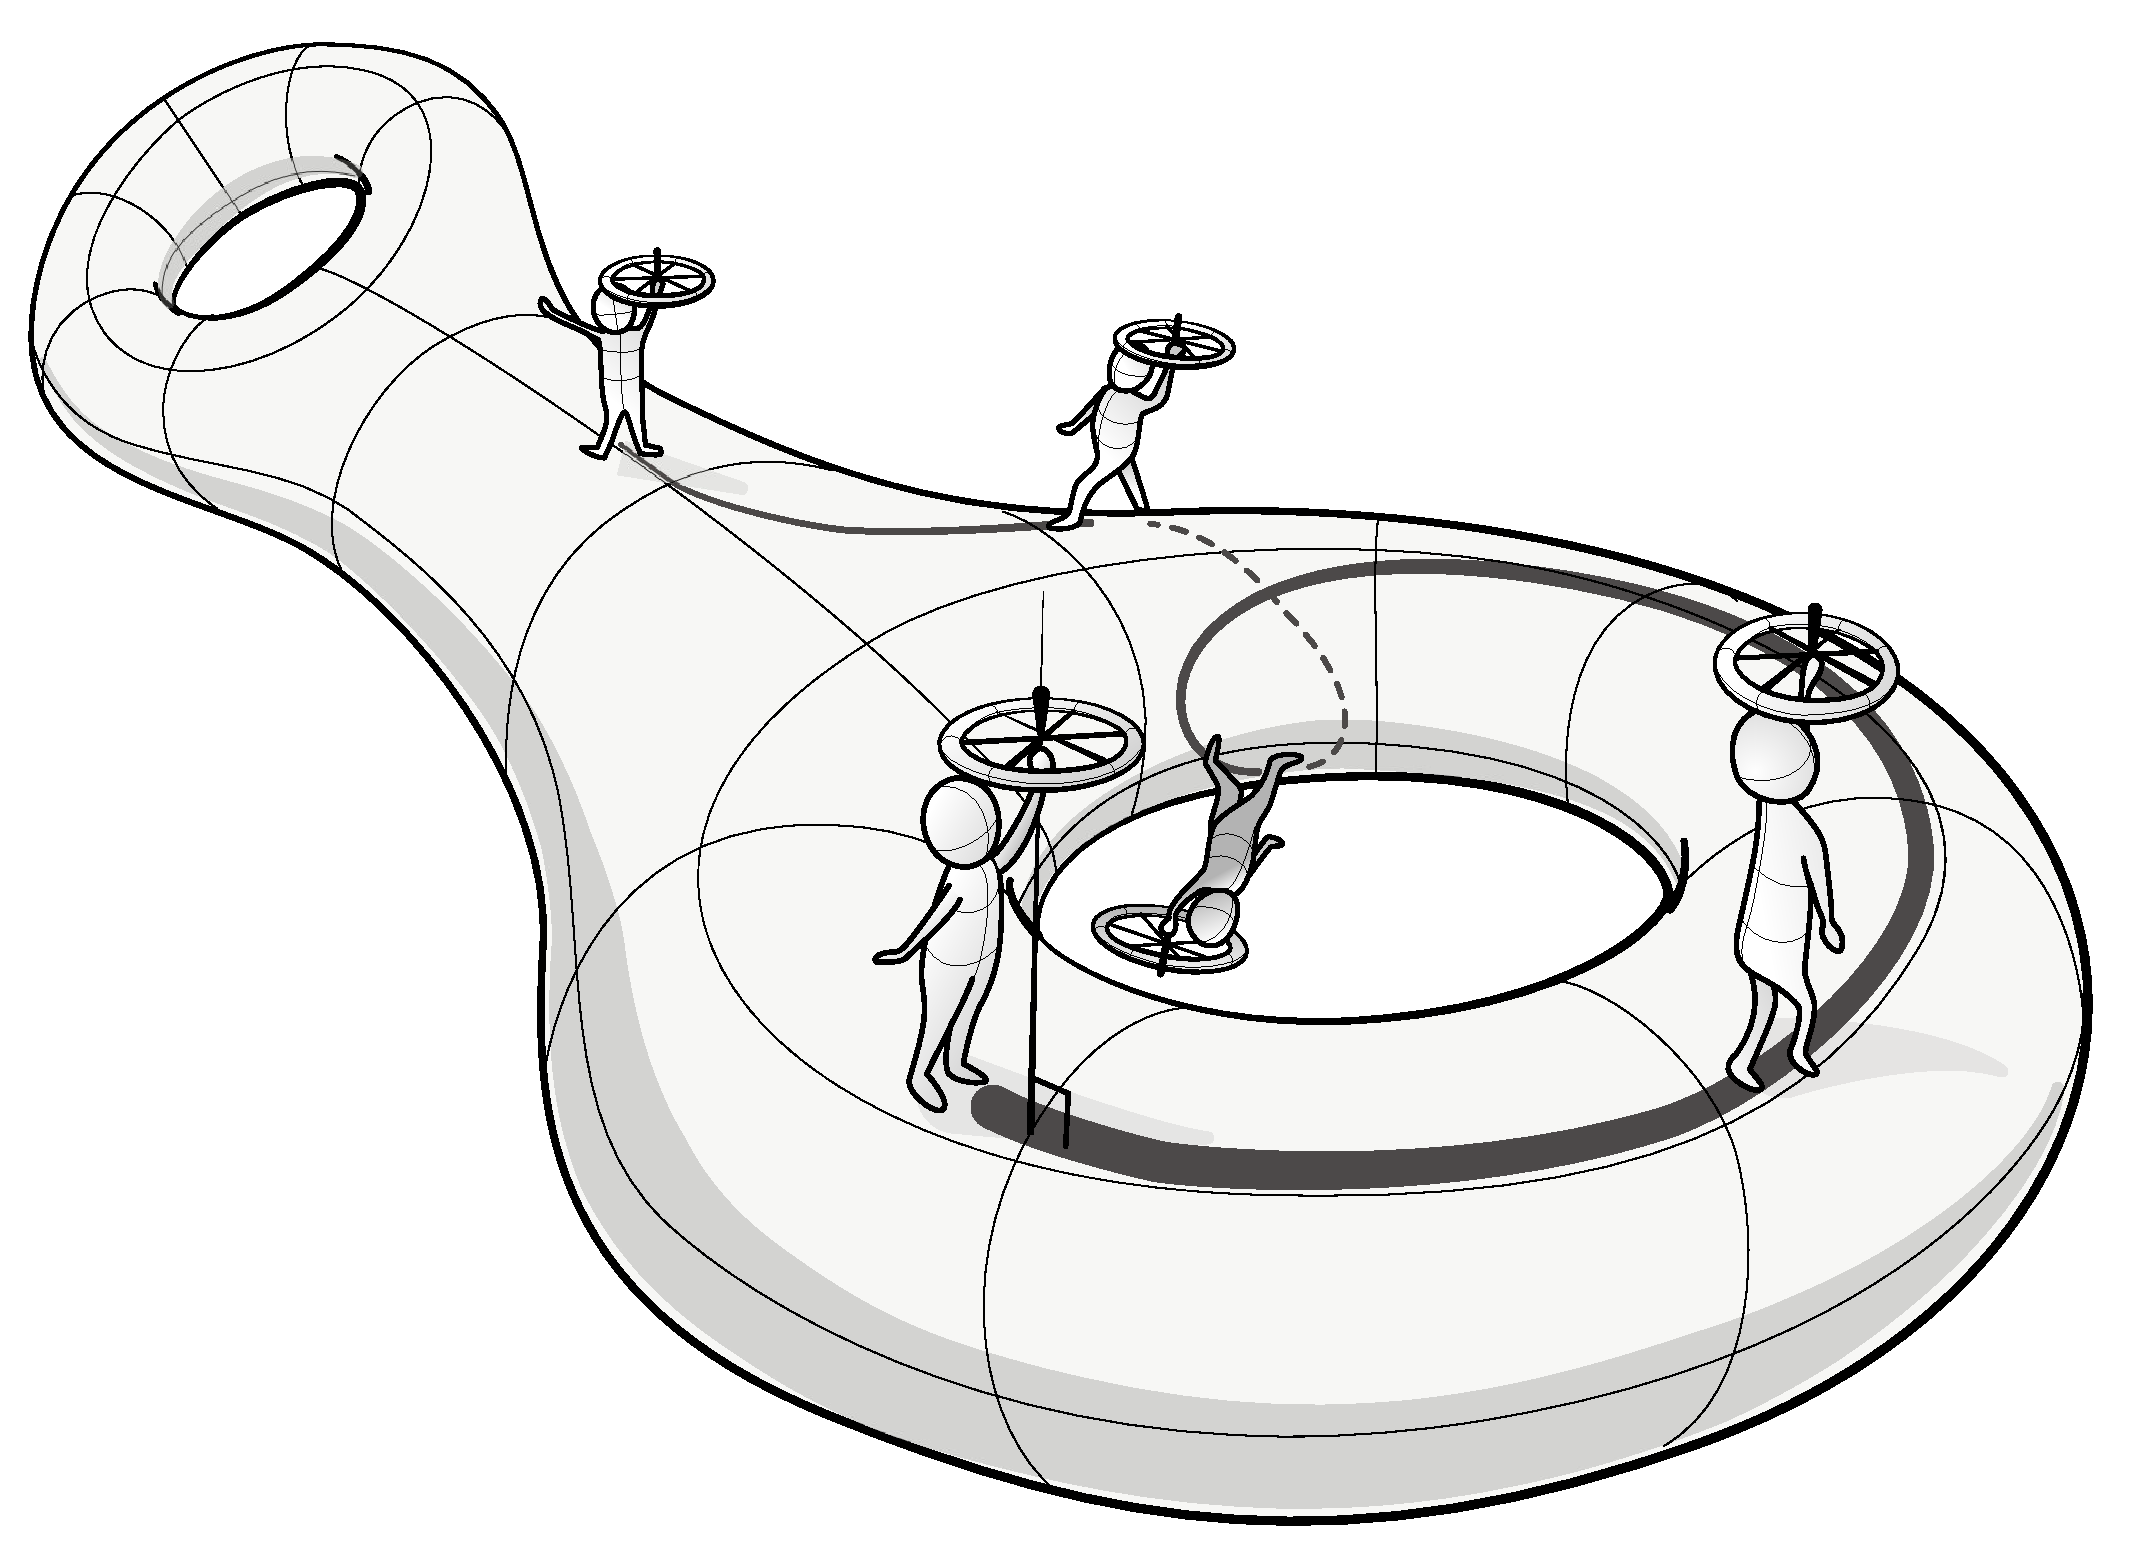
\includegraphics[scale=.3]{pics/parallel_transport}
\end{figure}

Пусть $\gamma\:[a,b]\to\Sigma$ --- гладкая кривая на гладкой поверхности $\Sigma$.
Представьте, что мы идём по поверхности вдоль $\gamma$, неся идеально сбалансированное велосипедное колесо.
При этом ось колеса всё время направлена перпендикулярно $\Sigma$ и мы не трогаем само колесо, держась только за его ось.
Если колесо не вращается в начальной точке $p\z=\gamma(a)$, то оно не будет вращаться после остановки в точке~$q=\gamma(b)$, ведь, прилагая силу к оси, нельзя придать колесу крутящий момент.
Тогда отображение, переводящее начальное положение колеса в конечное, и есть параллельный перенос~$\iota_\gamma$.

Между прочим, физическая интуиция должна подсказывать, что \textit{если не менять направление оси, то не будет меняться и направления спиц};
по сути это переформулировка наблюдения~\ref{obs:parallel=}.

Для второго толкования, выберем разбиение $a=t_0<\dots\z<t_n=b$ отрезка $[a,b]$
и рассмотрим последовательность ортогональных проекций $\phi_i\:\T_{\gamma(t_{i-1})}\to\T_{\gamma(t_i)}$.
Для достаточно мелкого разбиения композиция 
\[\phi_n\circ\dots\circ\phi_1\:\T_p\z\to\T_q\]
становится близкой к $\iota_\gamma$.

Каждая проекция $\phi_i$ не увеличивает длину векторов и то же верно для их композиции.
Однако, если разбиение достаточно мелкое, то композиция является почти изометрией.
А значит, предел $\iota_\gamma$ --- также изометрия $\T_p\z\to\T_q$.

\begin{thm}{Упражнение}\label{ex:holonomy=not0}
Постройте такую петлю $\gamma$ на $\mathbb{S}^2$, что параллельный перенос $\iota_\gamma$ не является тождественным отображением.
\end{thm}

\section{Полная геодезическая кривизна}

Напомним, что геодезическая кривизна определена в~\ref{sec:Darboux}.
Она обозначается через $k_g$ и измеряет, насколько кривая $\gamma$ на ориентированной поверхности отклоняется от геодезической;
если $\gamma$ поворачивает налево, то кривизна положительна, если направо, то отрицательна.
В частности, геодезические линии имеют нулевую геодезическую кривизну.

Пусть $\gamma\:\mathbb{I}\to \Sigma$ --- гладкая кривая с единичной скоростью на ориентированной гладкой поверхности $\Sigma$.
Полная геодезическая кривизна $\gamma$ определяется через интеграл 
\[\tgc\gamma=\tgc\gamma_\Sigma
\df
\int_{\mathbb{I}} k_g(t)\cdot dt.\]

Если $\Sigma$ --- это плоскость, то геодезическая кривизна $\gamma$ совпадает
с её ориентированной кривизной (см.~\ref{sec:Total signed curvature}).
В частности, её полная геодезическая кривизна равна её полной ориентированной кривизне.
По этой причине мы воспользовались тем же обозначением $\tgc\gamma$; если надо указать поверхность, то пишем $\tgc\gamma_\Sigma$.\index{10psi@$\tgc\gamma_\Sigma$ (полная геодезическая кривизна)}

Если $\gamma$ --- кусочно-гладкая кривая на $\Sigma$, то её \index{полная!геодезическая кривизна}\emph{полная геодезическая кривизна} определяется как сумма всех полных геодезических кривизн её дуг плюс сумма ориентированных внешних углов $\gamma$ на стыках.
Точнее, пусть $\gamma$ --- произведение гладких кривых $\gamma_1,\dots,\gamma_n$, тогда
\[\tgc\gamma
\df
\tgc{\gamma_1}+\dots+\tgc{\gamma_n}+\theta_1+\dots+\theta_{n-1},\]
где $\theta_i$ --- ориентированный внешний угол на стыке $\gamma_i$ и $\gamma_{i+1}$;
он положителен, если $\gamma$ поворачивает налево, и отрицателен, если $\gamma$ поворачивает направо; он не определён, если $\gamma$ поворачивает в противоположную сторону.
Если $\gamma$ замкнута, то 
\[\tgc\gamma
\df
\tgc{\gamma_1}+\dots+\tgc{\gamma_n}+\theta_1+\dots+\theta_n,\]
где $\theta_n$ --- это ориентированный внешний угол на стыке $\gamma_n$ и $\gamma_1$.

Если каждая дуга $\gamma_i$ в произведении является минимизирующей геодезической, то $\gamma$ называется \index{ломаная геодезическая}\emph{ломаной геодезической}.
В этом случае $\tgc{\gamma_i}=0$ для каждого~$i$.
Следовательно, полная геодезическая кривизна $\gamma$ равна сумме её ориентированных внешних углов.

\begin{thm}{Предложение}\label{prop:pt+tgc}
Пусть $\gamma$ --- замкнутая ломаная геодезическая на гладкой ориентированной поверхности $\Sigma$, которая начинается и заканчивается в точке~$p$.
Тогда параллельный перенос $\iota_\gamma\:\T_p\to\T_p$ представляет собой вращение по часовой стрелке плоскости $\T_p$ на угол~$\tgc\gamma$.

Утверждение остается верным для гладких замкнутых кривых и для кусочно-гладких кривых.
\end{thm}

\parbf{Доказательство.}
Пусть $\gamma$ --- циклическое произведение геодезических $\gamma_1,\dots,\gamma_n$.
Выберем касательный вектор ${\vec v}$ в точке $p$ и продолжим его до параллельного векторного поля вдоль~$\gamma$.
Поскольку поле $\tan_i(t)\z=\gamma_i'(t)$ параллельно вдоль $\gamma_i$, ориентированный угол $\phi_i$ от $\tan_i$ до ${\vec v}$ постоянен на каждой дуге~$\gamma_i$.

\begin{wrapfigure}{o}{22 mm}
\vskip-0mm
\centering
\includegraphics{mppics/pic-48}
\vskip-0mm
\end{wrapfigure}

Пусть $\theta_i$ --- внешний угол на стыке $\gamma_{i}$ и $\gamma_{i+1}$.
Тогда 
\[\phi_{i+1}=\phi_i-\theta_i \pmod{2\cdot\pi}.\]
Таким образом, после обхода всех вершин мы получаем, что 
\[\phi_{n+1}-\phi_1=-\theta_1-\dots-\theta_n=-\tgc\gamma \pmod{2\cdot\pi},\]
и первое утверждение следует.

Для гладкой кривой с единичной скоростью $\gamma\:[a,b]\to\Sigma$ доказательство аналогично.
Обозначим $\phi(t)$ как ориентированный угол от $\tan (t)$ до ${\vec v} (t)$.
Покажем, что 
\[\phi'(t)+k_g(t)\equiv0\eqlbl{eq:phi'+kg}\]

Напомним, что $\mu=\mu(t)$ --- это поворот $\tan \z=\tan(t)$ против часовой стрелки на угол $\tfrac\pi2$ в $\T_{\gamma(t)}$.
Обозначим через $\vec w=\vec w(t)$ поворот $\vec v=\vec v(t)$ против часовой стрелки на угол $\tfrac\pi2$ в $\T_{\gamma(t)}$.
Тогда
\begin{align*}
\tan&=\cos\phi\cdot \vec v-\sin\phi\cdot \vec w,
\\
\mu&=\sin\phi\cdot \vec v+\cos\phi\cdot \vec w.
\end{align*}

Векторные поля $\vec v$ и $\vec w$ параллельны вдоль $\gamma$; то есть $\vec v'(t),\vec w'(t)\z\perp\T_{\gamma(t)}$.
Следовательно, $\langle\vec v',\mu\rangle\z=\langle\vec w',\mu\rangle\z=0$.
Из этого следует, что
\begin{align*}
k_g&=\langle\tan',\mu\rangle=
\\
&=-(\sin^2\phi+\cos^2\phi)\cdot \phi'
\\
&=-\phi',
\end{align*}
что и доказывает \ref{eq:phi'+kg}.

Применив \ref{eq:phi'+kg}, получаем, что 
\begin{align*}
\phi(b)-\phi(a)&=\int_a^b \phi'(t)\cdot dt=
\\
&=-\int_a^b k_g\cdot dt=
\\
&=-\tgc\gamma
\end{align*}

Последний случай, когда $\gamma$ --- кусочно-гладкая кривая, результат доказывается прямым сочетанием доказательств двух рассмотренных случаев. 
\qeds
